\documentclass{ximera}

%\usepackage{todonotes}

\newcommand{\todo}{}

\usepackage{tkz-euclide}
\tikzset{>=stealth} %% cool arrow head
\tikzset{shorten <>/.style={ shorten >=#1, shorten <=#1 } } %% allows shorter vectors

\usepackage{tkz-tab}  %% sign charts
\usetikzlibrary{decorations.pathreplacing} 

\usetikzlibrary{backgrounds} %% for boxes around graphs
\usetikzlibrary{shapes,positioning}  %% Clouds and stars
\usetikzlibrary{matrix} %% for matrix
\usepgfplotslibrary{polar} %% for polar plots
\usetkzobj{all}
\usepackage[makeroom]{cancel} %% for strike outs
%\usepackage{mathtools} %% for pretty underbrace % Breaks Ximera
\usepackage{multicol}

\usepackage{polynom}



\usepackage[many]{tcolorbox}  %% for titled boxes
\newtcolorbox{xbox}[1]{%
    tikznode boxed title,
    enhanced,
    arc=0mm,
    interior style={white},
    attach boxed title to top center= {yshift=-\tcboxedtitleheight/2},
    fonttitle=\bfseries,
    colbacktitle=white,coltitle=black,
    boxed title style={size=normal,colframe=white,boxrule=0pt},
    title={#1}}


\usepackage{array}
\setlength{\extrarowheight}{+.1cm}   
\newdimen\digitwidth
\settowidth\digitwidth{9}
\def\divrule#1#2{
\noalign{\moveright#1\digitwidth
\vbox{\hrule width#2\digitwidth}}}





\newcommand{\RR}{\mathbb R}
\newcommand{\R}{\mathbb R}
\newcommand{\N}{\mathbb N}
\newcommand{\Z}{\mathbb Z}

%\renewcommand{\d}{\,d\!}
\renewcommand{\d}{\mathop{}\!d}
\newcommand{\dd}[2][]{\frac{\d #1}{\d #2}}
\newcommand{\pp}[2][]{\frac{\partial #1}{\partial #2}}
\renewcommand{\l}{\ell}
\newcommand{\ddx}{\frac{d}{\d x}}
\newcommand{\ddt}{\frac{d}{\d t}}

\newcommand{\zeroOverZero}{\ensuremath{\boldsymbol{\tfrac{0}{0}}}}
\newcommand{\inftyOverInfty}{\ensuremath{\boldsymbol{\tfrac{\infty}{\infty}}}}
\newcommand{\zeroOverInfty}{\ensuremath{\boldsymbol{\tfrac{0}{\infty}}}}
\newcommand{\zeroTimesInfty}{\ensuremath{\small\boldsymbol{0\cdot \infty}}}
\newcommand{\inftyMinusInfty}{\ensuremath{\small\boldsymbol{\infty - \infty}}}
\newcommand{\oneToInfty}{\ensuremath{\boldsymbol{1^\infty}}}
\newcommand{\zeroToZero}{\ensuremath{\boldsymbol{0^0}}}
\newcommand{\inftyToZero}{\ensuremath{\boldsymbol{\infty^0}}}



\newcommand{\numOverZero}{\ensuremath{\boldsymbol{\tfrac{\#}{0}}}}
\newcommand{\dfn}{\textbf}
%\newcommand{\unit}{\,\mathrm}
\newcommand{\unit}{\mathop{}\!\mathrm}
\newcommand{\eval}[1]{\bigg[ #1 \bigg]}
\newcommand{\seq}[1]{\left( #1 \right)}
\renewcommand{\epsilon}{\varepsilon}
\renewcommand{\iff}{\Leftrightarrow}

\DeclareMathOperator{\arccot}{arccot}
\DeclareMathOperator{\arcsec}{arcsec}
\DeclareMathOperator{\arccsc}{arccsc}
\DeclareMathOperator{\si}{Si}
\DeclareMathOperator{\proj}{proj}
\DeclareMathOperator{\scal}{scal}


\newcommand{\tightoverset}[2]{% for arrow vec
  \mathop{#2}\limits^{\vbox to -.5ex{\kern-0.75ex\hbox{$#1$}\vss}}}
\newcommand{\arrowvec}[1]{\tightoverset{\scriptstyle\rightharpoonup}{#1}}
\renewcommand{\vec}{\mathbf}
\newcommand{\veci}{\vec{i}}
\newcommand{\vecj}{\vec{j}}
\newcommand{\veck}{\vec{k}}
\newcommand{\vecl}{\boldsymbol{\l}}

\newcommand{\dotp}{\bullet}
\newcommand{\cross}{\boldsymbol\times}
\newcommand{\grad}{\boldsymbol\nabla}
\newcommand{\divergence}{\grad\dotp}
\newcommand{\curl}{\grad\cross}
%\DeclareMathOperator{\divergence}{divergence}
%\DeclareMathOperator{\curl}[1]{\grad\cross #1}


\colorlet{textColor}{black} 
\colorlet{background}{white}
\colorlet{penColor}{blue!50!black} % Color of a curve in a plot
\colorlet{penColor2}{red!50!black}% Color of a curve in a plot
\colorlet{penColor3}{red!50!blue} % Color of a curve in a plot
\colorlet{penColor4}{green!50!black} % Color of a curve in a plot
\colorlet{penColor5}{orange!80!black} % Color of a curve in a plot
\colorlet{fill1}{penColor!20} % Color of fill in a plot
\colorlet{fill2}{penColor2!20} % Color of fill in a plot
\colorlet{fillp}{fill1} % Color of positive area
\colorlet{filln}{penColor2!20} % Color of negative area
\colorlet{fill3}{penColor3!20} % Fill
\colorlet{fill4}{penColor4!20} % Fill
\colorlet{fill5}{penColor5!20} % Fill
\colorlet{gridColor}{gray!50} % Color of grid in a plot

\newcommand{\surfaceColor}{violet}
\newcommand{\surfaceColorTwo}{redyellow}
\newcommand{\sliceColor}{greenyellow}




\pgfmathdeclarefunction{gauss}{2}{% gives gaussian
  \pgfmathparse{1/(#2*sqrt(2*pi))*exp(-((x-#1)^2)/(2*#2^2))}%
}


%%%%%%%%%%%%%
%% Vectors
%%%%%%%%%%%%%

%% Simple horiz vectors
\renewcommand{\vector}[1]{\left\langle #1\right\rangle}


%% %% Complex Horiz Vectors with angle brackets
%% \makeatletter
%% \renewcommand{\vector}[2][ , ]{\left\langle%
%%   \def\nextitem{\def\nextitem{#1}}%
%%   \@for \el:=#2\do{\nextitem\el}\right\rangle%
%% }
%% \makeatother

%% %% Vertical Vectors
%% \def\vector#1{\begin{bmatrix}\vecListA#1,,\end{bmatrix}}
%% \def\vecListA#1,{\if,#1,\else #1\cr \expandafter \vecListA \fi}

%%%%%%%%%%%%%
%% End of vectors
%%%%%%%%%%%%%

%\newcommand{\fullwidth}{}
%\newcommand{\normalwidth}{}



%% makes a snazzy t-chart for evaluating functions
%\newenvironment{tchart}{\rowcolors{2}{}{background!90!textColor}\array}{\endarray}

%%This is to help with formatting on future title pages.
\newenvironment{sectionOutcomes}{}{} 



%% Flowchart stuff
%\tikzstyle{startstop} = [rectangle, rounded corners, minimum width=3cm, minimum height=1cm,text centered, draw=black]
%\tikzstyle{question} = [rectangle, minimum width=3cm, minimum height=1cm, text centered, draw=black]
%\tikzstyle{decision} = [trapezium, trapezium left angle=70, trapezium right angle=110, minimum width=3cm, minimum height=1cm, text centered, draw=black]
%\tikzstyle{question} = [rectangle, rounded corners, minimum width=3cm, minimum height=1cm,text centered, draw=black]
%\tikzstyle{process} = [rectangle, minimum width=3cm, minimum height=1cm, text centered, draw=black]
%\tikzstyle{decision} = [trapezium, trapezium left angle=70, trapezium right angle=110, minimum width=3cm, minimum height=1cm, text centered, draw=black]


\outcome{Use the first derivative to determine whether a function is increasing or decreasing.}
\outcome{Define higher order derivatives.}
\outcome{Compare differing notations for higher order derivatives.}
\outcome{Identify the relationships between the function and its first and second derivatives.}


\title[Dig-In:]{Higher order derivatives and graphs}

\begin{document}
\begin{abstract}
 Here we look at graphs of higher order derivatives.   
\end{abstract}
\maketitle

An important application of derivatives is in determining when a function is increasing or decreasing.
\begin{definition}\index{increasing}\index{decreasing}
	A function is \emph{increasing} on an interval $I$ if, for all $a$ and $b$ in the interval with $a<b$, then $f(a) < f(b)$.
	A function is \emph{decreasing} on an interval $I$ if, for all $a$ and $b$ in the interval with $a<b$, then $f(a) > f(b)$.
\end{definition}
\begin{example}
The following is the graph of $y=f(x)$.  On what intervals is $f$ increasing?  On what intervals is $f$ decreasing?
  \begin{image}
  \begin{tikzpicture}
	\begin{axis}[
            xmin=-2.1,xmax=3.1,ymin=-3,ymax=4,
            axis lines=center,
            width=6in,
            height=3in,
            every axis y label/.style={at=(current axis.above origin),anchor=south},
            every axis x label/.style={at=(current axis.right of origin),anchor=west},
          ]        
          \addplot [very thick,penColor,smooth, domain=(-2:3)] {(x^4)/4-(x^3)/3-x^2)};
        \end{axis}
  \end{tikzpicture}
  \end{image}
  \begin{explanation}
  	As we move along the graph from left to right, we see that the $y$-values are getting smaller until we get to $x=-1$.  Between $x=-1$ and $x=0$ the
	$y$-values are getting larger, then between $x=0$ and $x=2$ they get smaller again.  Finally, after $x=2$ they start growing.
	
	$f$ is increasing on: $(-1,\answer{0})$ and $(\answer{2},\infty)$.  $f$ is decreasing on $(-\infty, \answer{-1})$ and $(\answer{0}, \answer{2})$.
  \end{explanation}	
\end{example}

Let's look at each of the intervals from the last example separately.
On $(-\infty,-1)$, look at the slopes of the tangent lines.  Is there anything that all of those slopes have in common?
They are all NEGATIVE!  Look in the interval $(0,2)$.  The slopes are all negative in that interval as well.
What about in the interval $(1,0)$?  Those slopes are all POSITIVE.  Same for the interval $(2,\infty)$.
Notice that the positive slopes occurred when the function was increasing and the negative slopes occurred
when the function was decreasing?  That was no accident.

Since the derivative gives us a formula for the slope of a tangent
line to a curve, we can gain information about a function purely from
the sign of the derivative.  In particular, we have the following theorem
\begin{theorem}
  If $f$ is differentiable on an interval, then
\begin{itemize}
\item $f'(x)>0$ on that interval whenever $f$ is increasing as $x$
  increases on that interval.
\item $f'(x)<0$ on that interval whenever $f$ is decreasing as $x$
  increases on that interval.
\end{itemize}
\end{theorem}
\begin{question}
  Below we have graphed $y=f(x)$:
  \begin{image}
  \begin{tikzpicture}
	\begin{axis}[
            xmin=-2,xmax=2,ymin=-8,ymax=8,
            axis lines=center,
            width=6in,
            height=3in,
            every axis y label/.style={at=(current axis.above origin),anchor=south},
            every axis x label/.style={at=(current axis.right of origin),anchor=west},
          ]        
          \addplot [very thick,penColor,smooth, domain=(-2:2)] {x^3+x^2-2*x)};
        \end{axis}
  \end{tikzpicture}
  \end{image}
  Is the first derivative positive or negative on the interval $-1<x<1/2$?
  \begin{prompt}
    \begin{multipleChoice}
      \choice{Positive}
      \choice[correct]{Negative}
    \end{multipleChoice}
  \end{prompt}
\end{question}

\begin{question}
  Below we have graphed $y=f'(x)$:
  \begin{image}
  \begin{tikzpicture}
	\begin{axis}[
            xmin=-2,xmax=2,ymin=-8,ymax=8,
            axis lines=center,
            width=6in,
            height=3in,
            every axis y label/.style={at=(current axis.above origin),anchor=south},
            every axis x label/.style={at=(current axis.right of origin),anchor=west},
          ]        
          \addplot [very thick,penColor,smooth, domain=(-2:2)] {x^3+x^2-2*x)};
        \end{axis}
  \end{tikzpicture}
  \end{image}
  Is the graph of $f(x)$ increasing or decreasing as $x$ increases on
  the interval $-1<x<0$?
  \begin{prompt}
    \begin{multipleChoice}
      \choice[correct]{Increasing}
      \choice{Decreasing}
    \end{multipleChoice}
  \end{prompt}
\end{question}

We call the derivative of the derivative the \dfn{second
  derivative}, the derivative of the derivative of the derivative the
\dfn{third derivative}, and so on. We have special notation for
higher derivatives, check it out:
\begin{description}
\item[First derivative:] $\ddx f(x) = f'(x) = f^{(1)}(x)$.
\item[Second derivative:] $\dd[~^2]{x^2} f(x) = f''(x) = f^{(2)}(x)$.
\item[Third derivative:] $\dd[~^3]{x^3} f(x) = f'''(x) = f^{(3)}(x)$.
\end{description}

We use the facts above in our next example.

\begin{example}
  Here we have unlabeled graphs of $f$, $f'$, and $f''$:
  \begin{image}
  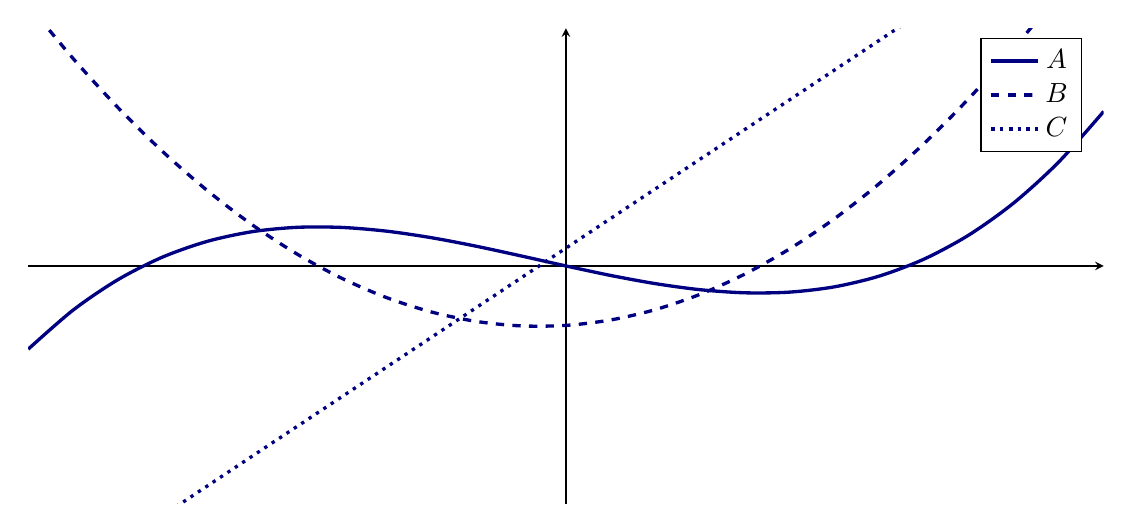
\begin{tikzpicture}
	\begin{axis}[
            xmin=-2,xmax=2,ymin=-8,ymax=8,
            axis lines=center,
            ticks=none,
            width=6in,
            height=3in,
            every axis y label/.style={at=(current axis.above origin),anchor=south},
            every axis x label/.style={at=(current axis.right of origin),anchor=west},
          ]        
          \addplot [very thick,penColor,smooth, domain=(-2:2)] {x^3+.3*x^2-2*x)};
          \addlegendentry{$A$};
          \addplot [very thick, dashed,penColor,smooth, domain=(-2:2)] {3*x^2+2*.3*x-2)};
          \addlegendentry{$B$};
          \addplot [very thick, dotted,penColor,smooth, domain=(-2:2)] {6*x+2*.3)};
          \addlegendentry{$C$};
        \end{axis}
  \end{tikzpicture}
  \end{image}
  Identify each curve above as a graph of $f$, $f'$, or $f''$.
  \begin{explanation} 
    Here we see three curves, $A$, $B$, and $C$. Since $A$ is
    \wordChoice{\choice{positive} \choice{negative}
      \choice[correct]{increasing} \choice{decreasing}} when $B$ is
    positive and
    \wordChoice{\choice{positive}\choice{negative}\choice{increasing}\choice[correct]{decreasing}}
    when $B$ is negative, we see
    \[
    A'=B.
    \]
    Since $B$ is increasing when $C$ is
    \wordChoice{\choice[correct]{positive}\choice{negative}\choice{increasing}
      \choice{decreasing}} and decreasing when $C$ is
    \wordChoice{\choice{positive}\choice[correct]{negative}\choice{increasing}\choice{decreasing}}, we see
    \[
    B'=C.
    \]
    Hence $f=A$, $f'=B$, and $f''=C$.
  \end{explanation}
\end{example}




\begin{example}
    Here we have unlabeled graphs of $f$, $f'$, and $f''$:
    \begin{image}
      \begin{tikzpicture}
	\begin{axis}[
            domain=-4:4,
            ticks=none,
            ymax=2, ymin=-2,
            xmax=4, xmin=-4,
            axis lines =middle,
            every axis y label/.style={at=(current axis.above origin),anchor=south},
            every axis x label/.style={at=(current axis.right of origin),anchor=west},
            width=6in,
            height=3in,
          ]
          \addplot [very thick, penColor,smooth,samples=100] {2/(.75*sqrt(2*pi))*exp(-((x)^2)/(2*.75^2)) *(-x)/(.75^2)};
          \addlegendentry{$A$};
          \addplot [very thick, dashed,penColor,smooth,samples=100] {2*gauss(0,.75)};
          \addlegendentry{$B$};
          \addplot [very thick, dotted,penColor,smooth,samples=100] {2/(.75*sqrt(2*pi))*exp(-((x)^2)/(2*.75^2)) *(-1)/(.75^2) +
            2/(.75*sqrt(2*pi))*exp(-((x)^2)/(2*.75^2)) *(x^2)/(.75^4)};
          \addlegendentry{$C$};
        \end{axis}
          \end{tikzpicture}
\end{image}
    Identify each curve above as a graph of $f$, $f'$, or $f''$.
      \begin{explanation} 
        Here we see three curves, $A$, $B$, and $C$. Since $B$ is
        \wordChoice{\choice{positive}\choice{negative}\choice[correct]{increasing}\choice{decreasing}} when $A$
        is positive and
        \wordChoice{\choice{positive}\choice{negative}\choice{increasing}\choice[correct]{decreasing}} when $A$
        is negative, we see
        \[
        B'=A.
        \]
        Since $A$ is increasing when $C$ is
        \wordChoice{\choice[correct]{positive}\choice{negative}\choice{increasing}\choice{decreasing}}
          and decreasing when $C$ is
          \wordChoice{\choice{positive}\choice[correct]{negative}\choice{increasing}\choice{decreasing}}, we
          see
        \[
        A'=C.
        \]
        Hence $f=\answer[given]{B}$, $f'=\answer[given]{A}$, and
        $f''=\answer[given]{C}$.
      \end{explanation}
\end{example}

\begin{example}
  Here we have unlabeled graphs of $f$, $f'$, and $f''$:
  \begin{image}
  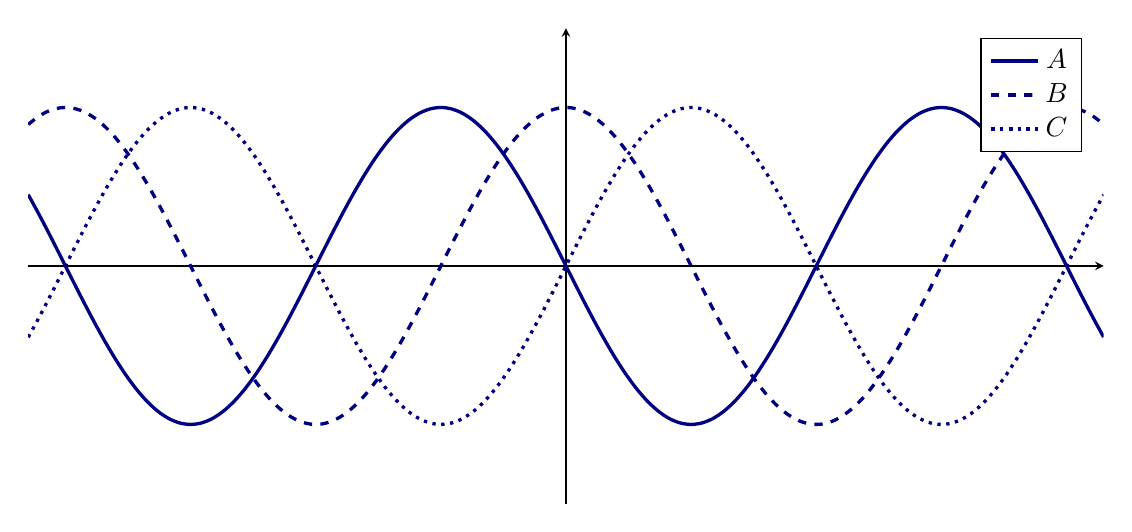
\begin{tikzpicture}
	\begin{axis}[
            xmin=-6.75,xmax=6.75,ymin=-1.5,ymax=1.5,
            axis lines=center,
            ticks=none,
            width=6in,
            height=3in,
            every axis y label/.style={at=(current axis.above origin),anchor=south},
            every axis x label/.style={at=(current axis.right of origin),anchor=west},
          ]        
          \addplot [very thick, penColor, samples=100,smooth, domain=(-6.75:6.75)] {-sin(deg(x))};
          \addlegendentry{$A$};
          \addplot [very thick, dashed,penColor, samples=100,smooth, domain=(-6.75:6.75)] {cos(deg(x))};
          \addlegendentry{$B$};
          \addplot [very thick, dotted,penColor, samples=100,smooth, domain=(-6.75:6.75)] {sin(deg(x))};
          \addlegendentry{$C$};
        \end{axis}
  \end{tikzpicture}
  \end{image}
  Identify each curve above as a graph of $f$, $f'$, or $f''$.
  %One is of $f$, another is of $f'$ and a third is of $f''$.  Explain
  %what strategies you could use to identify which graph corresponds
    \begin{explanation} %%BADBAD Need Dropdown
    Here we see three curves, $A$, $B$, and $C$. Since $C$ is
    \wordChoice{\choice{positive}\choice{negative}\choice[correct]{increasing}\choice{decreasing}} when $B$ is
    positive and \wordChoice{\choice{positive}\choice{negative}\choice{increasing}\choice[correct]{decreasing}}
    when $B$ is negative, we see
    \[
    C'=B.
    \]
    Since $B$ is increasing when $A$ is
    \wordChoice{\choice[correct]{positive}\choice{negative}\choice{increasing}\choice{decreasing}} and
    decreasing when $A$ is
    \wordChoice{\choice{positive}\choice[correct]{negative}\choice{increasing}\choice{decreasing}}, we see
    \[
    B'=A.
    \]
    Hence $f=\answer[given]{C}$, $f'=\answer[given]{B}$, and
    $f''=\answer[given]{A}$.
  \end{explanation}
\end{example}


\end{document}
